% CREATED BY DAVID FRISK, 2016
\chapter{Theory and Technologies} \label{ch2} 
In this chapter, we first review the preliminary notions of Computational Linguistics relevant to this work. 
We then give a more rigorous definition of the problem at hand and present the basic idea behind our proposed automation approach, comparing it to the existing ones and mentioning the technologies involved.

\section{Preliminary notions}
This first section consists of an overview of the basic notions that are necessary for a full understanding of the approach we propose. 
First, we discuss the principle of compositionality. 
After that, we describe and compare the grammar formalisms involved in the project, focussing on the two playing the most prominent roles in this work and comparing them to other, related approaches.

\subsection{Semantic compositionality}
The principle of semantic compositionality states, in its most general form, that the meaning of a complex expression is determined solely by the meanings of its components and by the manner in which these components are combined \cite{frege}. \smallskip 

A useful variant of this formulation, which refers to natural languages in particular, is the following: \smallskip

\begin{definition} \label{sc}
For every complex expression $e$ in a language $L$, the meaning of $e$ in $L$ is determined by the structure of $e$ and the meanings of the constituents of $e$ in $L$.
\end{definition}
\smallskip

Questions of structure and constituency are settled by the syntax of $L$, while the meanings of simple expressions are given by the lexical semantics of $L$, meaning that syntax and lexical semantics, together, are sufficient to determine the entire semantics of $L$ \cite{frege}. \smallskip

According to this definition, then, if $L$ is compositional, the meaning of an expression $e$ in $L$ cannot depend directly on the context in which $S$ is used in or on the intentions of the speaker who uses it, even though it might be the case that the meanings of the constituents of $e$ depend on the context or on the speaker's intentions, thus making the sentence indirectly depend on them \cite{semcom2}. \smallskip

While many artificial languages, such as programming languages, are compositional by construction, the general validity of this principle for natural languages is, despite many arguments in favor, under debate. 
In this work, we make the assumption that compositionality also holds for natural languages, or at least that it is a useful notion applying to most natural language sentences\footnote{In Section \ref{evalign}, however, we will see that idiomatic expressions, often used as an arguments against compositionality, are also challenging to deal with in the context of grammar-based CA.}. \smallskip

In particular, we adapt the notion of semantic compositionality to translation. 
The intuitive idea is that the translation of a sentence is composed of translations of each part of the original one. Adjusting Definition \ref{sc}:

\begin{definition}
    For every complex expression $e$ in a source language $S$, the translation of $e$ in a target language $T$ is determined by the structure of $e$ and the translations of the constituents of $e$ in $T$.
\end{definition}

\subsection{Constituency grammars}
The idea of taking advantage of semantic compositionality is not new in the field of Computational Linguistics. 
Doing so traditionally involves using some kind of \textit{constituency grammar}. \smallskip

The notion of constituency or \textit{phrase structure} grammar, introduced by Noam Chomsky in \cite{chomsky}, is usually known to computer scientists due to the fact that a class of phrase structure grammars, namely that of \textit{Context-Free Grammars} (CFGs), that can be used to describe programming languages and plays an central role in compiler theory. 
As a consequence, we find giving a complete formal definition of the latter unnecessary and will restrict ourselves to an informal review of the aspects that are particularly relevant for the specific subject of this thesis. \smallskip

A constituency grammar consists essentially in a set of \textit{rewrite rules}, such as 

\begin{lstlisting}[frame=none]
    S -> NP VP,
\end{lstlisting}

which we can read as ``$S$ can be \textit{rewritten as} (or \textit{substituted with}) a $\mathit{NP}$ followed by a $\mathit{VP}$'', or as ``a sentence $S$ is constituted by a noun phrase $\mathit{NP}$ and a verb phrase $\mathit{VP}$''. \smallskip

\begin{figure}[h]
    \centering
    \begin{subfigure}{.35\textwidth}
      \centering
      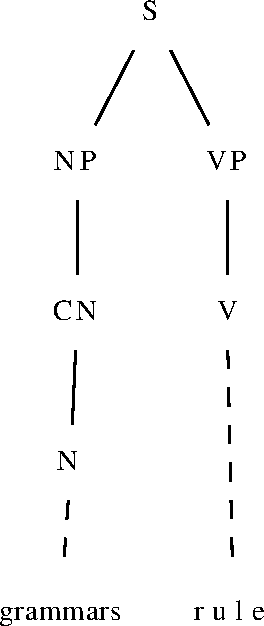
\includegraphics[width=.4\linewidth]{figure/parsetree.pdf}
    \end{subfigure}%
    \begin{subfigure}{.6\textwidth}
        \centering
        \begin{lstlisting}
            S -> NP VP
            NP -> CN
            VP -> V
            CN -> N
            N -> "grammars"
            V -> "rule"
        \end{lstlisting}
    \end{subfigure}
    \caption[Parse tree of the sentence ``\textit{grammars rule}'' and corresponding grammar fragment]{Parse tree of the simple sentence ``\textit{grammars rule}''. On the right, the fragment of the simple but linguistically informed grammar necessary to obtain such tree.}
    \label{pt}
\end{figure}

Replacing the term ``constituted'' with ``composed'' makes it easy to understand in which way phrase structure grammars are related to the aforementioned principle of compositionality. \smallskip

In the context of MT, the idea of exploiting the constituency relation and, as such, compositionality, was proposed by Curry in the early 1960s \cite{curry61} and first put in practice two decades later in the form of an experimental interlingual translation system, not coincidentally named Rosetta, which requires the definition of two distinct logically isomorphic \textit{Montague grammars}\footnote{Montague grammars are a semantics-oriented development of \textit{categorial grammars}, which are in turn a type of constituency grammars.} - one for the Source Language (SL), one for the Target Language (TL) - and constructs an intermediate representation based on such isomorphism \cite{rosetta}. \smallskip

\subsubsection{Synchronous grammars}
Among constituency grammars, other formalisms that have been employed in more recent MT systems are that of \textit{synchronous CFG}, originally developed for programming language compilation \cite{scfg} and adapted to natural language translation in several settings \cite{nlpscfg0,nlpscfg1,nlpscfg2,nlpscfg3}, and, later on, that of \textit{synchronous TAG} \cite{stag}, a variation of \textit{TAG} (Tree-Adjoining Grammar) \cite{tag}.
Both formalisms are meant to characterize correspondences between languages by having as their elements, instead of single rewrite rules, pairs of rules - one for the source and one for the target language. 
In a synchronous TAG, the constituents of a SL rule may be linked to their counterparts in the corresponding TL rule, and such links may be used to identify concepts in a syntax-based fashion. \smallskip

\subsubsection{Grammatical Framework} \label{gf}
% translation as compilation
As the repeated mention of programming language compilers in the above may suggest, it is possible to draw a very close parallel between compiler and MT pipelines. From this perspective, a natural language translation system can consist of: \smallskip

\begin{itemize}
    \item a \textit{frontend}, where the SL is analyzed or \textit{parsed} and whose output is an \textit{intermediate representation} most frequently in the form of an \textit{Abstract Syntax Tree} (AST)
    \item a \textit{backend}, where the AST is \textit{linearized} by means of application of a set of rules, a process usually referred to as \textit{code generation} in the context of programming languages and that we will refer to as \text{Target Language Generation} (TLG) or, when the context makes it clear that what the TL is, \textit{Natural Language Generation} (NLG). \smallskip
\end{itemize}
\begin{figure}[H]
    \centering
    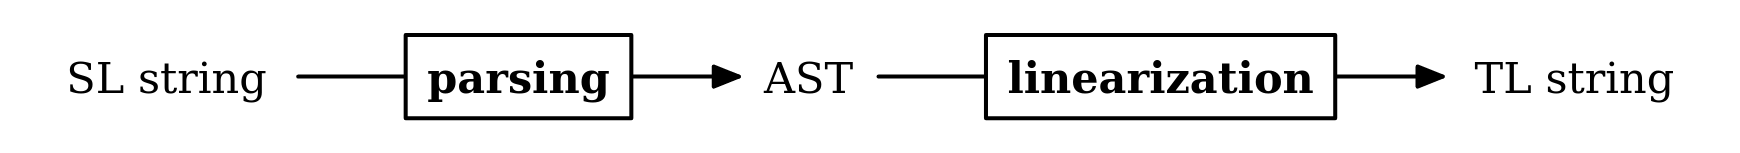
\includegraphics[width=.8\linewidth]{figure/compiler.png}
    \caption[Steps of programming language compilation and, in the case of GF, natural language translation]{Steps of programming language compilation and, in the case of GF, natural language translation. In compilation, the input is usually a high-level programming language and the output is machine code (or code in a lower-level language). In the case of MT, the input and the output are strings in two different natural languages.} \label{compilerd}
\end{figure}

% intro to GF
Grammatical Framework (GF), being a grammar formalism and programming language designed with this parallel in mind, goes a step further in the direction of synchronous CFGs and TAGs. 
It introduces in fact a clear distinction between the \textit{abstract syntax}, whose aim is to capture the syntactic structures all natural languages taken into account have in common, and the \textit{concrete syntaxes}, specific to each individual language, consisting in their linearization rules \cite{gf2004} \cite{gfbook}. 
This makes it possible to deal with multiple languages by writing only one grammar, whose components are an abstract syntax and several concrete syntaxes, providing a solid basis for a system able to translate between any pair of for which a concrete syntax is available, in any direction. \smallskip

% GF as an interlingua-based MT system
With respects to this, GF can be also seen as an \textit{interlingual} MT system where the intermediate representation or \textit{interlingua} is an AST. Interlingua-based systems have the advantage, in terms of efficiency, of making it unnecessary to build $n (n - 1)$ translation functions to cover all possible pairs of $n$ languages: having $2n$ is in general enough. In GF in particular, using a multilingual grammar makes it so that translation can be performed, for each pair of languages, in both directions, so that $n$ translation functions (or rahter $n$ concrete syntaxes and an abstract syntax) are already sufficient.\smallskip

% the RGL
An advantage of GF in particular, in addition, is the availability of a set of \textit{resource grammars} - the Resource Grammar Library (RGL) - for a variety of languages. A resource grammar is essentially a grammar that captures only the syntactic and morphological structures of a language, i.e. a grammar in the traditional sense of the term, and that can be easily extended to construct what is usually referred to as an \textit{application grammar}, i.e. a domain-specific grammar aiming to describe the language in a way that is not only syntactically correct, but also semantically accurate \cite{gfbook}. \smallskip

% GF and xMT
Extending the RGL in various ways, translation experiments with GF grammars have been conducted in the field of eXplainable Machine Translation (XMT), as the ASTs produced by SL analysis can serve both as to some extent automatically checkable certificates for the correctness of translation - by backlinearization to the SL - and as fully inspectable explanations aimed towards expert users \cite{rantaxmt}. \smallskip

% limitations
While the approach described above has proved successful for domain-specific translation, i.e. in cases where the natural languages in question can be reduced to \textit{Constrained Natural Languages} (CNLs), when it comes to open-domain translation, while target language generation remains effective, the results are negatively affected by the lack of robustness of the GF-based parsers available at the time of writing.

\subsection{Dependency grammars} \label{depg}
% DGs as opposed to PSGs
A class of grammar formalisms alternative to phrase structure, first proposed in \cite{dg}, is that of \textit{dependency grammars}, the main difference between the two being the relation they are based on. 
As opposed to constituency, \textit{dependency} is a word-to-word correspondence, meaning that words are simply put in relation with each other via directed links, called in fact \textit{dependencies}. 
Each dependency is, then, composed of two words: a \textit{head} and a \textit{dependent} that refers to it. For instance, if we try to look at syntactic dependencies in the sentence ``\textit{grammars rule}'', we could identify the verb ``\textit{rule}'' as the head and the noun ``\textit{grammars}'', its subject, as its dependent. \smallskip 

% pros
Intuitively, this means that dependency trees are simpler than their phrase structure counterparts. This makes them an easier target for the frontend, possibly ML-based, of a MT system such as the one outlined in the above. 
Existing \textit{dependency parsers}, such as UDPipe \cite{udpipe1} and the Standford parser \cite{standford}, are often - but not always \cite{rasp} - neural pipelines trained on dependency treebanks, significantly more robust than their phrase structure counterparts. 

% cons
On the other hand, there is currently no effective way to use these trees as a starting point for NLG: dependency grammars are an effective way to describe language, but, unlike phrase-structure grammars, they are not \textit{generative},\footnote{That does not mean, however, that dependency grammars have not been made use of in MT research, in conjunction with statistical techniques, in order to better capture grammatical generalizations \cite{treelet}.}. \smallskip

One idea is, then, to develop a hybrid system where the frontend is a dependency parser and the backend a grammaticality-preserving GF-based target language generation module. 
This work goes in this direction, and the connecting link between these two seemingly incompatible stages of the pipeline is, as we will elaborate on in Section \ref{ourapproach}, a CA component able to identify matching dependency trees and generate the corresponding GF concrete and abstract syntax functions: concepts.

While there are several different dependency-based frameworks, the following section focuses on the one we find most well suited to this purpose, \textit{Universal Dependencies}. 

\subsubsection{Universal Dependencies} \label{ud} 
Universal Dependencies (UD) is a framework for cross-linguistically consistent grammatical annotation. 
The UD project aims at developing parallel treebanks for many languages in order to support, among other things, the development of multilingual dependency parsers, such as the aforementioned UDPipe \cite{udpipe1}. 
In order to do so, it specifies an annotation scheme and a standard format for dependency trees consisting in an evolution of (universal) Stanford dependencies \cite{st1, st2}, Google universal part-of-speech tags \cite{upos}, and the Interset interlingua for morphosyntactic tagsets \cite{tagconv}. 
The basic idea behind such standard is to provide a set of Part-Of-Speech (POS) tags, dependency relations and annotation guidelines as language-agnostic as possible - so to facilitate its application in multilingual settings - while allowing language-specific extensions whenever necessary. \smallskip

In the following, we give a quick overview of the standard format UD uses to store dependency trees and of the aspects of the annotation scheme that are most relevant to the task at hand. 
Appendix \ref{a} provides a more comprehensive, but not completely exhaustive, description of all the POS tags and dependency labels mentioned in the examples appearing in this work based on that in \cite{compsyn}. 
The reader interested in a full specification of the UD annotation scheme may refer to the official UD documentation\footnote{Available at \url{universaldependencies.org}.}. 

\paragraph{The CoNLL-U format} \label{conll}
The standard plain text format for dependency trees, CoNLL-U, is an extension of CoNNL-X \cite{conllx} which may contain \textit{comment lines}, starting with \texttt{\#}, \textit{blank lines} marking sentence boundaries and \textit{word lines} containing the annotation of a single token (generally a word, with some exceptions\footnote{Examples of such exceptions are Italian contractions such as ``\textit{dello}'', which is generally divided into ``\textit{del}'' + ``\textit{lo}''.} in 10 tab-separated fields: \smallskip

\begin{enumerate}
    \item \texttt{ID}: integer\footnote{Again, there are exceptions: in the case of Italian contractions and other multiword tokens, ranges may be used. Furthermore, empty nodes are characterized by decimal numbers between 0 and 1.} representing the position of the word in the sentence, starting from 1
    \item \texttt{FORM}: inflected from of the word
    \item \texttt{LEMMA}: lemmatized form of the word
    \item \texttt{UPOS}: universal POS tag
    \item \texttt{XPOS}: language-specific POS tag (optional)
    \item \texttt{FEATS}: list of (universal or language-specific) morphological features (optional)
    \item \texttt{HEAD}: head of the current word, i.e. either the value of the \texttt{ID} of another word in the same sentence or 0 in case the word at hand is a \texttt{root}
    \item \texttt{DEPREL}: universal dependency relation to the \texttt{HEAD} (\texttt{root} in case the word at hand is itself the \texttt{root})
    \item \texttt{DEPS}: enhanced dependency graph in the form of a list of \texttt{HEAD}-\texttt{DEPREL} pairs (optional)
    \item \texttt{MISC}: any other annotation (optional)
\end{enumerate} \smallskip

\begin{figure}[h]
    \centering
    \begin{subfigure}{.55\textwidth}
      \centering
      \footnotesize
        \begin{verbatim}
1	this	this	PRON	_	_	5	nsubj	_	_
2	is	be	AUX	_	_	5	cop	_	_
3	a	a	DET	_	_	5	det	_	_
4	dependency	dependency	NOUN	_	_	5	compound	_	_
5	tree	tree	NOUN	_	_	0	root	_	_
        \end{verbatim}
    \end{subfigure}%
    \begin{subfigure}{.45\textwidth}
        \centering
        \footnotesize
        \setlength{\unitlength}{0.21mm}
        \begin{picture}(371.0,130.0)
            \put(0.0,0.0){this}
            \put(46.0,0.0){is}
            \put(83.0,0.0){a}
            \put(120.0,0.0){dependency}
            \put(220.0,0.0){tree}
            \put(0.0,15.0){{\tiny PRON}}
            \put(46.0,15.0){{\tiny AUX}}
            \put(83.0,15.0){{\tiny DET}}
            \put(120.0,15.0){{\tiny NOUN}}
            \put(220.0,15.0){{\tiny NOUN}}
            \put(120.0,30.0){\oval(218.63636363636363,133.33333333333334)[t]}
            \put(10.681818181818187,35.0){\vector(0,-1){5.0}}
            \put(105.0,99.66666666666667){{\tiny nsubj}}
            \put(143.0,30.0){\oval(172.27586206896552,100.0)[t]}
            \put(56.86206896551724,35.0){\vector(0,-1){5.0}}
            \put(128.0,83.0){{\tiny cop}}
            \put(161.5,30.0){\oval(134.8102189781022,66.66666666666667)[t]}
            \put(94.0948905109489,35.0){\vector(0,-1){5.0}}
            \put(146.5,66.33333333333334){{\tiny det}}
            \put(180.0,30.0){\oval(97.0,33.333333333333336)[t]}
            \put(131.5,35.0){\vector(0,-1){5.0}}
            \put(165.0,49.66666666666667){{\tiny compound}}
            \put(235.0,130.0){\vector(0,-1){100.0}}
            \put(240.0,120.0){{\tiny root}}
        \end{picture}
    \end{subfigure}
    \caption[A dependency tree in CoNNL-U format alongside its graphical representation]{A dependency tree in CoNNL-U format alongside its graphical representation. Optional fields in the CoNLL-U file are left blank.}
\end{figure}

\paragraph{Universal POS tags} \label{upos}
Universal POS tags mark the core part-of-speech categories, such as nouns, verbs, pronouns and determiners. \smallskip

An important distinction we can make based on POS tags is, as we will see in Section \ref{criteria}, that between \textit{content} and \textit{function} words.
\textit{Content} or \textit{open class} words are words with a lexical meaning (nouns, lexical verbs, adjectives, adverbs and interjections).
\textit{Function} words, like pronouns and determiners, only have a grammatical meaning. Since they do not readily accept new members\footnote{One exception is the recent introduction of the gender-neutral pronoun ``\textit{hen}'' in Swedish.}, they are often referred to also as \textit{closed class} words. \smallskip

While the majority of Universal POS tags correspond to the grammatical categories of traditional grammars, the UD annotation scheme does have its peculiarities. 
Most importantly for the following discussion, verbs are divided into lexical verbs, tagged \texttt{VERB}, and auxiliaries, tagged \texttt{AUX}, thus providing an easy way to distinguish between content verbs and function verbs. 
A more systematic description of \texttt{UPOS} tags is given in \ref{a_pos}.

\paragraph{Universal dependency relations}
%subtypes
Universal dependency relations, largely based on \cite{st2}, represent, as mentioned in the above, syntactic dependencies between individual pairs of words occurring in the same sentence. 
In particular, according to the CoNLL-U standard (cf. Section \ref{conll}), each word is assigned a \textit{dependency label} indicating in which way it is liked to its \texttt{HEAD}. \smallskip 

In this sense, the only exceptional case, which will be the starting point for our short overview of dependency relations, is that of the \texttt{root} label, generally assigned to the main verb of a sentence, ignoring any auxiliaries. 
For instance, ``\textit{smoked}'' is the root of the sentence \smallskip

\begin{example} \label{katia1}
    ``Katia has just \underline{smoked} a cigarette''
\end{example} \smallskip

In cases such as the following, where the main verb is a copula, the root is its complement and the verb is linked to it with the label \texttt{cop}. \smallskip

\begin{example} \label{katia2}
    ``Katia is a \underline{psychologist}''
\end{example} \smallskip

 If a sentence contains is no verbs at all, there is no fixed rule excepts that, in order to avoid unnecessary discrepancies between languages, the root should be a content word. \smallskip

\begin{figure}[h]
   \centering
   \scriptsize
   \begin{subfigure}{.5\textwidth}
        \centering
        \setlength{\unitlength}{0.24mm}
        \begin{picture}(380.0,110.0)
            \put(0.0,0.0){Katia}
            \put(55.0,0.0){has}
            \put(92.0,0.0){just}
            \put(138.0,0.0){smoked}
            \put(202.0,0.0){a}
            \put(239.0,0.0){cigarette}
            \put(0.0,15.0){{\tiny PROPN}}
            \put(55.0,15.0){{\tiny AUX}}
            \put(92.0,15.0){{\tiny ADV}}
            \put(138.0,15.0){{\tiny VERB}}
            \put(202.0,15.0){{\tiny DET}}
            \put(239.0,15.0){{\tiny NOUN}}
            \put(79.0,30.0){\oval(135.82608695652175,100.0)[t]}
            \put(11.086956521739125,35.0){\vector(0,-1){5.0}}
            \put(64.0,83.0){{\tiny nsubj}}
            \put(106.5,30.0){\oval(79.3855421686747,66.66666666666667)[t]}
            \put(66.80722891566265,35.0){\vector(0,-1){5.0}}
            \put(91.5,66.33333333333334){{\tiny aux}}
            \put(125.0,30.0){\oval(39.47826086956522,33.333333333333336)[t]}
            \put(105.26086956521739,35.0){\vector(0,-1){5.0}}
            \put(110.0,49.66666666666667){{\tiny advmod}}
            \put(230.5,30.0){\oval(28.89189189189189,33.333333333333336)[t]}
            \put(216.05405405405406,35.0){\vector(0,-1){5.0}}
            \put(215.5,49.66666666666667){{\tiny det}}
            \put(208.5,30.0){\oval(98.02970297029702,66.66666666666667)[t]}
            \put(257.5148514851485,35.0){\vector(0,-1){5.0}}
            \put(193.5,66.33333333333334){{\tiny obj}}
            \put(153.0,110.0){\vector(0,-1){80.0}}
            \put(158.0,100.0){{\tiny root}}
          \end{picture}
   \end{subfigure}%
   \begin{subfigure}{.5\textwidth}
        \centering
        \setlength{\unitlength}{0.20mm}
        \begin{picture}(474.0,150.0)
            \put(0.0,0.0){Katia}
            \put(55.0,0.0){has}
            \put(92.0,0.0){worked}
            \put(156.0,0.0){in}
            \put(193.0,0.0){a}
            \put(230.0,0.0){big}
            \put(267.0,0.0){school}
            \put(331.0,0.0){library}
            \put(0.0,15.0){{\tiny PROPN}}
            \put(55.0,15.0){{\tiny AUX}}
            \put(92.0,15.0){{\tiny VERB}}
            \put(156.0,15.0){{\tiny ADP}}
            \put(193.0,15.0){{\tiny DET}}
            \put(230.0,15.0){{\tiny ADJ}}
            \put(267.0,15.0){{\tiny NOUN}}
            \put(331.0,15.0){{\tiny NOUN}}
            \put(56.0,30.0){\oval(88.73913043478261,66.66666666666667)[t]}
            \put(11.630434782608695,35.0){\vector(0,-1){5.0}}
            \put(41.0,66.33333333333334){{\tiny nsubj}}
            \put(83.5,30.0){\oval(28.89189189189189,33.333333333333336)[t]}
            \put(69.05405405405405,35.0){\vector(0,-1){5.0}}
            \put(68.5,49.66666666666667){{\tiny aux}}
            \put(253.5,30.0){\oval(173.28571428571428,133.33333333333334)[t]}
            \put(166.85714285714286,35.0){\vector(0,-1){5.0}}
            \put(238.5,99.66666666666667){{\tiny case}}
            \put(272.0,30.0){\oval(135.82608695652175,100.0)[t]}
            \put(204.08695652173913,35.0){\vector(0,-1){5.0}}
            \put(257.0,83.0){{\tiny det}}
            \put(290.5,30.0){\oval(98.02970297029702,66.66666666666667)[t]}
            \put(241.4851485148515,35.0){\vector(0,-1){5.0}}
            \put(275.5,66.33333333333334){{\tiny amod}}
            \put(309.0,30.0){\oval(59.3125,33.333333333333336)[t]}
            \put(279.34375,35.0){\vector(0,-1){5.0}}
            \put(294.0,49.66666666666667){{\tiny compound}}
            \put(231.5,30.0){\oval(237.744769874477,166.66666666666666)[t]}
            \put(350.3723849372385,35.0){\vector(0,-1){5.0}}
            \put(216.5,116.33333333333333){{\tiny obl}}
            \put(107.0,150.0){\vector(0,-1){120.0}}
            \put(112.0,140.0){{\tiny root}}
          \end{picture}
   \end{subfigure}
   \begin{subfigure}{.4\textwidth}
        \centering
        \setlength{\unitlength}{0.2mm}
        \begin{picture}(277.0,110.0)
            \put(0.0,0.0){Katia}
            \put(55.0,0.0){is}
            \put(92.0,0.0){a}
            \put(129.0,0.0){psychologist}
            \put(0.0,15.0){{\tiny PROPN}}
            \put(55.0,15.0){{\tiny AUX}}
            \put(92.0,15.0){{\tiny DET}}
            \put(129.0,15.0){{\tiny NOUN}}
            \put(74.5,30.0){\oval(126.67441860465117,100.0)[t]}
            \put(11.162790697674417,35.0){\vector(0,-1){5.0}}
            \put(59.5,83.0){{\tiny nsubj}}
            \put(102.0,30.0){\oval(69.94594594594595,66.66666666666667)[t]}
            \put(67.02702702702703,35.0){\vector(0,-1){5.0}}
            \put(87.0,66.33333333333334){{\tiny cop}}
            \put(120.5,30.0){\oval(28.89189189189189,33.333333333333336)[t]}
            \put(106.05405405405405,35.0){\vector(0,-1){5.0}}
            \put(105.5,49.66666666666667){{\tiny det}}
            \put(144.0,110.0){\vector(0,-1){80.0}}
            \put(149.0,100.0){{\tiny root}}
          \end{picture}
   \end{subfigure}%
   \begin{subfigure}{.6\textwidth}
        \centering
        \setlength{\unitlength}{0.2mm}
        \begin{picture}(530.0,110.0)
            \put(0.0,0.0){Katia}
            \put(55.0,0.0){showed}
            \put(119.0,0.0){me}
            \put(165.0,0.0){a}
            \put(202.0,0.0){book}
            \put(248.0,0.0){about}
            \put(303.0,0.0){the}
            \put(340.0,0.0){Stone}
            \put(395.0,0.0){Age}
            \put(0.0,15.0){{\tiny PROPN}}
            \put(55.0,15.0){{\tiny VERB}}
            \put(119.0,15.0){{\tiny PRON}}
            \put(165.0,15.0){{\tiny DET}}
            \put(202.0,15.0){{\tiny NOUN}}
            \put(248.0,15.0){{\tiny ADP}}
            \put(303.0,15.0){{\tiny DET}}
            \put(340.0,15.0){{\tiny PROPN}}
            \put(395.0,15.0){{\tiny PROPN}}
            \put(37.5,30.0){\oval(49.54545454545455,33.333333333333336)[t]}
            \put(12.727272727272727,35.0){\vector(0,-1){5.0}}
            \put(22.5,49.66666666666667){{\tiny nsubj}}
            \put(107.0,30.0){\oval(59.3125,33.333333333333336)[t]}
            \put(136.65625,35.0){\vector(0,-1){5.0}}
            \put(92.0,49.66666666666667){{\tiny iobj}}
            \put(193.5,30.0){\oval(28.89189189189189,33.333333333333336)[t]}
            \put(179.05405405405406,35.0){\vector(0,-1){5.0}}
            \put(178.5,49.66666666666667){{\tiny det}}
            \put(148.5,30.0){\oval(144.9591836734694,66.66666666666667)[t]}
            \put(220.9795918367347,35.0){\vector(0,-1){5.0}}
            \put(133.5,66.33333333333334){{\tiny obj}}
            \put(304.0,30.0){\oval(88.73913043478261,66.66666666666667)[t]}
            \put(259.6304347826087,35.0){\vector(0,-1){5.0}}
            \put(289.0,66.33333333333334){{\tiny case}}
            \put(331.5,30.0){\oval(28.89189189189189,33.333333333333336)[t]}
            \put(317.05405405405406,35.0){\vector(0,-1){5.0}}
            \put(316.5,49.66666666666667){{\tiny det}}
            \put(217.5,30.0){\oval(283.94736842105266,100.0)[t]}
            \put(359.47368421052636,35.0){\vector(0,-1){5.0}}
            \put(202.5,83.0){{\tiny obl}}
            \put(387.5,30.0){\oval(49.54545454545455,33.333333333333336)[t]}
            \put(412.27272727272725,35.0){\vector(0,-1){5.0}}
            \put(372.5,49.66666666666667){{\tiny flat}}
            \put(70.0,110.0){\vector(0,-1){80.0}}
            \put(75.0,100.0){{\tiny root}}
          \end{picture}
    \end{subfigure}
      
   \caption[UD trees showing the common dependency relations that are discussed in Chapter \ref{ch3}]{UD trees showing the common dependency relations that are discussed in Chapter \ref{ch3}. The three on the left correspond to examples \ref{katia1} and \ref{katia2}.}
    \label{katia}
\end{figure}

Other dependency labels commonly found in simple clauses and that will be dwelt on in Chapter \ref{ch3}, all exemplified in Figure \ref{katia}, are: \smallskip
\begin{itemize}
    \item \texttt{nsubj}, marking the link between a noun, proper noun, pronoun or numeral to the \texttt{root} of a sentence or, more in general, to the head of a clause
    \item \texttt{aux}, marking auxiliary verbs other than the copula
    \item \texttt{obj}, \texttt{iobj} and \texttt{obl} marking the link between a verb and its object, indirect object and other complements respectively
    \item \texttt{advmod}, \texttt{amod}, \texttt{nummod} and \texttt{nmod}, marking links between modifiers and the nouns or verbs they refer to
    \item \texttt{flat}, indicating a flat multiword expression, and \texttt{compound}, appearing in compound nouns whenever they are written as two or more separate words.
\end{itemize} \smallskip

A more detailed description of all the UD labels mentioned in this work is given in \ref{a_lab}. 
However, because the topic will arise in Chapter \ref{ch3}, it is also worth mentioning that CoNNL-U trees can present UD labels followed by a \textit{subtype}, separated by the label itself by a semicolon and used to indicate grammatical relations that are specific to one language or a small group of related languages. A subtype that is commonly used in English is, for instance, \texttt{pass}, added to both the (clausal or nominal) syntactic subject and \texttt{aux} of a sentence in passive voice.

\begin{figure}[h]
    \centering
    \begin{subfigure}{.5\textwidth}
        \centering
        \setlength{\unitlength}{0.25mm}
\begin{picture}(259.0,90.0)
  \put(0.0,0.0){Katia}
  \put(55.0,0.0){reads}
  \put(110.0,0.0){a}
  \put(147.0,0.0){magazine}
  \put(0.0,15.0){{\tiny PROPN}}
  \put(55.0,15.0){{\tiny VERB}}
  \put(110.0,15.0){{\tiny DET}}
  \put(147.0,15.0){{\tiny NOUN}}
  \put(37.5,30.0){\oval(49.54545454545455,33.333333333333336)[t]}
  \put(12.727272727272727,35.0){\vector(0,-1){5.0}}
  \put(22.5,49.66666666666667){{\tiny nsubj}}
  \put(138.5,30.0){\oval(28.89189189189189,33.333333333333336)[t]}
  \put(124.05405405405405,35.0){\vector(0,-1){5.0}}
  \put(123.5,49.66666666666667){{\tiny det}}
  \put(121.0,30.0){\oval(88.73913043478261,66.66666666666667)[t]}
  \put(165.3695652173913,35.0){\vector(0,-1){5.0}}
  \put(106.0,66.33333333333334){{\tiny obj}}
  \put(70.0,90.0){\vector(0,-1){60.0}}
  \put(75.0,80.0){{\tiny root}}
\end{picture}
    \end{subfigure}%
    \begin{subfigure}{.5\textwidth}
        \centering
        \setlength{\unitlength}{0.25mm}
        \begin{picture}(344.0,90.0)
            \put(0.0,0.0){A}
            \put(37.0,0.0){magazine}
            \put(119.0,0.0){is}
            \put(156.0,0.0){read}
            \put(202.0,0.0){by}
            \put(239.0,0.0){Katia}
            \put(0.0,15.0){{\tiny DET}}
            \put(37.0,15.0){{\tiny NOUN}}
            \put(119.0,15.0){{\tiny AUX}}
            \put(156.0,15.0){{\tiny VERB}}
            \put(202.0,15.0){{\tiny ADP}}
            \put(239.0,15.0){{\tiny PROPN}}
            \put(28.5,30.0){\oval(28.89189189189189,33.333333333333336)[t]}
            \put(14.054054054054054,35.0){\vector(0,-1){5.0}}
            \put(13.5,49.66666666666667){{\tiny det}}
            \put(106.5,30.0){\oval(116.47899159663865,66.66666666666667)[t]}
            \put(48.260504201680675,35.0){\vector(0,-1){5.0}}
            \put(91.5,66.33333333333334){{\tiny nsubj:pass}}
            \put(147.5,30.0){\oval(28.89189189189189,33.333333333333336)[t]}
            \put(133.05405405405406,35.0){\vector(0,-1){5.0}}
            \put(132.5,49.66666666666667){{\tiny aux:pass}}
            \put(230.5,30.0){\oval(28.89189189189189,33.333333333333336)[t]}
            \put(216.05405405405406,35.0){\vector(0,-1){5.0}}
            \put(215.5,49.66666666666667){{\tiny case}}
            \put(217.5,30.0){\oval(79.3855421686747,66.66666666666667)[t]}
            \put(257.1927710843373,35.0){\vector(0,-1){5.0}}
            \put(202.5,66.33333333333334){{\tiny obl}}
            \put(171.0,90.0){\vector(0,-1){60.0}}
            \put(176.0,80.0){{\tiny root}}
          \end{picture}
    \end{subfigure}
    \caption[The UD trees of an example active sentence and its passive counterpart]{The UD trees of an example active sentence and its passive counterpart.}
    \label{actpass}
\end{figure}

\paragraph{Relation to GF} \label{udrelgf}
The complementarity of constituency and dependency grammars and the multilingual nature of UD make it interesting to use in conjunction with GF, and experiments aimed at exploiting their similarities have already been performed \cite{gfud, udgf}. 
In the case of hybrid MT pipelines as the one sketched in Section \ref{depg}, UD trees need to be at some point converted into GF ASTs, albeit with the disadvantage that, unlike its reverse, the UD-to-GF conversion is a non-deterministic search problem.
An algorithm for conversion in this direction is presented in \cite{udgf}, where \texttt{gf-ud}, a program for converting GF ASTs into UD trees initially presented in \cite{gfud}, is extended to also be able to do the reverse. 

\begin{figure}[h]
    \centering
    \begin{subfigure}{.7\textwidth}
        \centering
        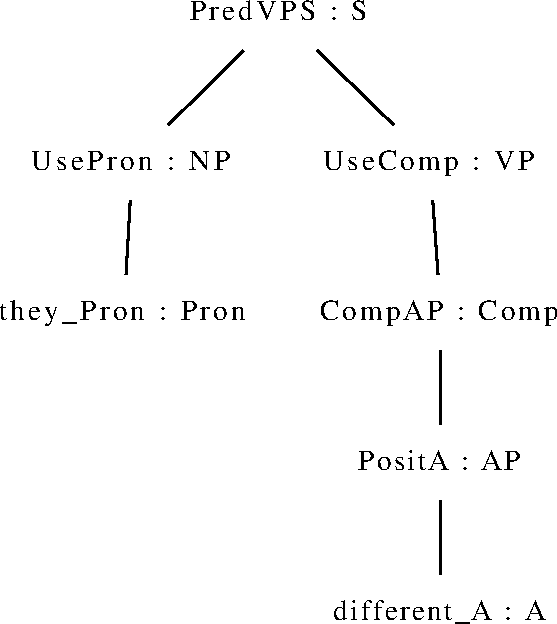
\includegraphics[width=.4\linewidth]{figure/different.pdf}
    \end{subfigure}%
    \begin{subfigure}{.3\textwidth}
        \centering
        \setlength{\unitlength}{0.25mm}
        \begin{picture}(194.0,90.0)
          \put(0.0,0.0){they}
          \put(46.0,0.0){are}
          \put(83.0,0.0){different}
          \put(0.0,15.0){{\tiny PRON}}
          \put(46.0,15.0){{\tiny AUX}}
          \put(83.0,15.0){{\tiny ADJ}}
          \put(51.5,30.0){\oval(79.3855421686747,66.66666666666667)[t]}
          \put(11.807228915662648,35.0){\vector(0,-1){5.0}}
          \put(36.5,66.33333333333334){{\tiny nsubj}}
          \put(74.5,30.0){\oval(28.89189189189189,33.333333333333336)[t]}
          \put(60.054054054054056,35.0){\vector(0,-1){5.0}}
          \put(59.5,49.66666666666667){{\tiny cop}}
          \put(98.0,90.0){\vector(0,-1){60.0}}
          \put(103.0,80.0){{\tiny root}}
        \end{picture}
    \end{subfigure}
    \caption[A GF AST and its UD counterpart]{A GF AST and its UD counterpart. Note how the copula is implicit in the GF AST and subordinate to its complement in UD.}
    \label{parsetree}
\end{figure}


\section{Concept Alignment}
In this section, we aim to give an exhaustive description of CA and of the subtasks it consists of. In order to do that, we deem it necessary to start by giving a definition of what we commonly refer to as \textit{concepts}. 

\subsection{Concepts} \label{concepts}
Intuitively, concepts are the components of meaning, and therefore, in a multilingual context, the units of translation. 
If we assume the principle of compositionality to be valid and apply it to translation, these meaning components are the common denominator between an expression in the source language and its translation, which can be generated using them as the starting point. \smallskip

From the compiler-like perspective described in Section \ref{gf}, this means that concepts are what the abstract syntax should represent, i.e. that they \textit{are} the ``interlingua'' of the MT system. 
This raises the question of how to obtain the abstract syntax needed for GF-based MT starting from a corpus of parallel texts, and it is at this point that language comparison and, as such, CA, come into play.

\subsection{Alignments} \label{aligns}
In terms of parallel text analysis, an \textit{alignment} consists in a pair of semantically equivalent (i.e., in this context, sharing the same abstract syntax) concrete expressions, one in the source and one in the target language. 
Even though, unless otherwise specified, we will keep referring to \textit{language pairs}, with a source and a target language, it is easy to see how this can be generalized to a more-than-bilingual, multidirectional definition.
The pair just mentioned simply becomes a tuple of equivalent expressions in different languages. Formally, \smallskip

\begin{definition} \label{algndef}
    An $n$-lingual \textit{alignment} is an $n$-uple $\langle e_1,...,e_n \rangle$ of semantically equivalent expressions, where each expressions $e_i$ is in a different language $L_i$.
\end{definition} \smallskip

While this general definition does not specify it, expressions are not necessarily represented as strings, but can rather be defined as tree-like structures, and in the present case as dependency trees that can later be replaced by GF ASTs. Matching ASTs can finally be used to generate the rules of a multilingual GF grammar, as we will discuss in Chapter \ref{ch5}. \smallskip

As mentioned in the Introduction, the task of aligning concepts comes in two variants:
\begin{enumerate}
    \item \textbf{\textit{Concept Extraction}} (CE), which consists in identifying new concepts via linguistic comparison and whose output is a set of bilingual alignments
    \item \textbf{\textit{Concept Propagation}} (CP), i.e. the task of finding the concrete expressions corresponding to a set of known concepts in a particular language. Here, by concepts we do not mean necessarily ASTs, as a suitable approach is to propagate UD tree alignments before obtaining the corresponding abstract representation.
\end{enumerate} \smallskip

If, as in the case of this project, the aim is to develop a multilingual MT system, these two tasks can be seen as two potentially subsequent steps. A first objective, in fact, can be to extract a set of concepts by comparing two translations of the same text. Once these concepts are in adequate number and of sufficient quality, it becomes possible to provide support for additional languages by simply looking for the concrete expressions that, in the new language, correspond to each of the previously gathered concepts. In other situations, clearly, CE alone can be enough or, if a set of concepts is already known, CP can be applied independently from CE to find their equivalents in a new language.

\subsection{Approaches to automation} 
Some form of manual, semi- or fully automated CA is in a sense at the heart of all traditional, even very early, MT systems. 
In the following section, we review some standard approaches. After discussing their limitations, we conclude the chapter with an overview of the grammar-based approach proposed in this thesis.

\subsubsection{Existing methods} \label{statmt}  
In the simplest case, \textit{word alignment} consists in finding pairs of individual words that translate to each other and store them in a dictionary. 
The standard automatic approaches to this task are statistical, and among them the five IBM Models \cite{ibm} and their numerous variations stand out. 
The IBM Models are a sequence of increasingly complex alignment models \cite{bitext}: \smallskip

\begin{itemize}
    \item Model 1 is based exclusively on lexical translation probabilities
    \item Model 2 takes word order (i.e. the absolute word positions) into account 
    \item Model 3 takes even a \textit{fertility} parameter into account (fertility being the number of target words that can be generated from a given source word)
    \item Models 4 and 5 take the \textit{context} (i.e. the relative position of the words) in which each word occurs into account in a broader sense
\end{itemize}

The GIZA++ toolkit \cite{gizapp}, an open source implementation of the IBM models based on the initial GIZA package \cite{giza}, is widely used, for instance in SMT systems such as Moses \cite{moses}. \smallskip

As mentioned in the Introduction, however, alignment can be performed at different levels of abstraction: to bring this to the extreme, there are contexts in which we might want to align full sentences, or even whole documents. While the latter two levels of abstraction are not necessarily relevant to MT, only aligning individual words is also, as discussed in the Introduction, not always the best option. For this reason, word alignment is often generalized to \textit{phrase alignment}. In systems like GIZA++, whose output is a list of pairs of word positions indicating which words in the SL string are to be aligned with which words in the TL string (commonly referred to as the \textit{pharaoh format}), extracting phrase alignments by combining the indices is realtively straightforward. \smallskip 

\begin{figure}[h]
    \centering
    \begin{subfigure}{.55\textwidth}
      \centering
      \footnotesize
      \begin{itemize}
          \item[SL] ``\textit{Word alignment with standard statistical tools}''
          \item[TL] ``\textit{Allineamento parola per parola con strumenti statistici standar}''
      \end{itemize}
    \end{subfigure}%
    \begin{subfigure}{.45\textwidth}
        \centering
        \footnotesize
        \setlength{\unitlength}{0.21mm}
        \begin{verbatim}
    0-1 0-2 0-3 1-0 2-4 3-7 4-6 5-5
        \end{verbatim}
    \end{subfigure}
    \footnotesize
    \smallskip
    \smallskip
    \begin{itemize}
        \item \texttt{0-1 0-2 0-3}: $\langle$\textit{``word'', ``parola per parola''}$\rangle$
        \item \texttt{1-0}: $\langle$\textit{``alignment'', ``allineamento''}$\rangle$
        \item \texttt{2-4}: $\langle$\textit{``with'', ``con''}$\rangle$
        \item \texttt{3-7}: $\langle$\textit{``standard'', ``standard''}$\rangle$
        \item \texttt{4-6}: $\langle$\textit{``statistical'', ``statistici''}$\rangle$
        \item \texttt{5-5}: $\langle$\textit{``tools'', ``strumenti''}$\rangle$
        \item \texttt{0-1 0-2 0-3 1-0}: $\langle$\textit{``word alignment'', ``allineamento parola per parola''}$\rangle$
        \item ...
    \end{itemize}
    ...
    \caption[The pharaoh format output of optimal word alignment on a pair of Italian-English sentences and some derived phrase alignments]{The pharaoh format output of optimal word alignment on a pair of Italian-English sentences and, below, some of the phrase alignments that can be derived from it.}
    \label{wordalgn}
\end{figure}

However, it must be noted that, in the context of statistical MT, the term ``phrase'' is not to be intended in its grammatical sense, but can refer to any sequence of - typically contiguous - words. 
In any case, both for word and phrase alignment, the relation that is established with these statistical methods is merely between strings in different languages: there is no intermediate representation capturing the concepts themselves. \smallskip

The parallel between MT and compiler pipelines proposed in Section \ref{gf} suggests instead that a more flexible approach, applicable at any level of abstraction, could be grammar-based. 
This is particularly useful in cases, not at all uncommon, where the minimal translation units are, in one or both the source and the target language, multiword - potentially discontinuous - expressions or even more complex constructions that phrase alignment is not able to handle. \smallskip 

Over time, various constituency grammar-based approaches have been proposed \cite{t2t1, t2t2}. 
These approaches, which make use of parallel treebanks, can be referred to as \textit{tree-to-tree alignment} methods \cite{bitext}. 
While theoretically appealing, however, their use in data-driven MT is limited, since they tend to suffer not only from the scarce availability of large-scale manually annotated corpora and the lack of robustness of the existing parsers, but also from the fact that, in general, the monolingual grammars used for parsing tend to be designed independently from each other, following different traditions, formalisms and linguistic theories \cite{nlphandbook}, thus making it often impossible to find a common representation describing a complete mapping from one tree to another \cite{bitext}.

\subsubsection{Our approach} \label{ourapproach}
Given that GF solves the latter problem, that it provides a good basis for NLG and that the intermediate representations it makes use of preserve all the syntactic information present in a sentence, the idea of trying to perform CA by comparing GF ASTs seems tempting. 
However, since ASTs need to be obtained from raw - or, at most, barely sentence-segmented - text, CA would suffer from the same problem that, as mentioned in in Section \ref{gf}, affects other tree-to-tree alignment methods and GF-based open-domain translation: the lack of a sufficiently robust analysis stage and, as a consequence, the inadequacy of the resulting parse trees. \smallskip

As anticipated throughout this chapter, we attempt to solve this problem by taking advantage of dependency parsing. 
In particular, UD is our formalism of choice since its focus on ``universality'' (i.e. on abstracting away from cross-lingual differences) makes it as interesting as GF itself when it comes to the possibility of establishing mappings between trees in different languages. 
Furthermore, when it comes to MT itself, using UD allows us to take advantage of the tools that have been developed to leverage its similarities with GF (cf. Section \ref{ud}), thus enabling GF target language generation. \smallskip

Concretely, this means that the system we propose requires the following elements, whose reciprocal relations are shown in Figure \ref{elems}: \smallskip

\begin{itemize}
    \item a UD parser
    \item an alignment module based on dependency tree comparison, which is the tangible output of this project and whose CE and CP components are described and evaluated in detail in Chapters \ref{ch3} and \ref{ch4} respectively
    \item a program, based on \texttt{gf-ud}, that converts the alignments into GF ASTs to then generate a domain-specific GF lexicon\footnote{CA is performed on UD trees, i.e. before conversion to GF, to reduce the possibility of errors. The reason is that, as mentioned in Section \ref{udrelgf}, in fact, such conversion is not obtained by means of a deterministic procedure and, as such, is not always guaranteed to be correct.}.
\end{itemize} \smallskip

The CE and CP modules are implemented as part of the project, while the UD parser and \texttt{gf-ud} are independently developed open source software, even though the latter, being currently under development was adapted and extended as part of the process. 
In addition, we provide a simple GF-based translation script to evaluate the performance of the CA module to the test.

\begin{figure}[h]
    \centering
    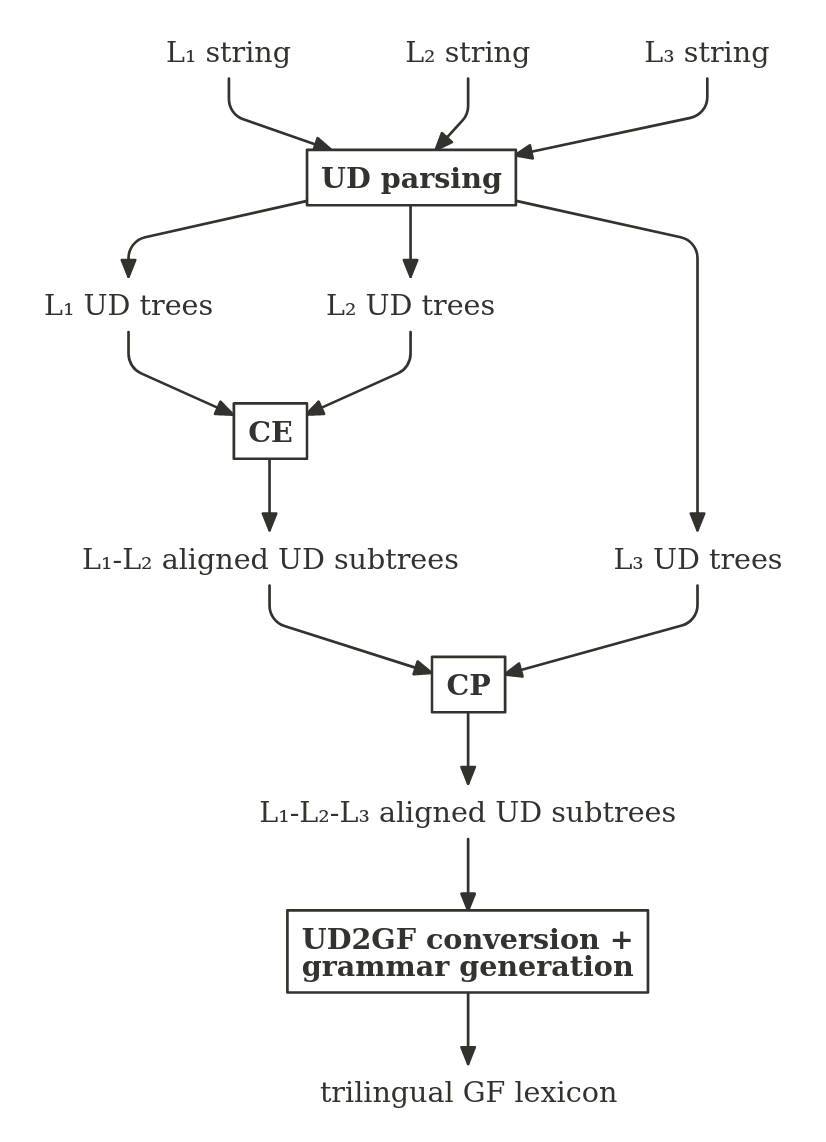
\includegraphics[width=.6\linewidth]{figure/elems.png}
    \caption[Relationship between the different components of the CA system]{Relationship between the different components of the system proposed in this work. The diagram shows the minimal, trilingual use case in which both CE and CP can be made use of.} \label{elems}
    \label{sys}
\end{figure}
